\documentclass[a4paper, 12pt]{paper}

\usepackage{BMETeX_BSc}
\usepackage{fancyvrb}
\usepackage{tocloft}
\usepackage{algorithm}
\usepackage{algpseudocode}
\usepackage{multirow}
\newlength\longest
\renewcommand{\tableshortname}{Table}
\makeatletter
\def\BState{\State\hskip-\ALG@thistlm}
\makeatother

\VerbatimFootnotes
\bibliographystyle{IEEEtranN}
\begin{document}

\pagenumbering{Roman} % Roman numbering
\begin{center}
    \begin{figure}[!h]
        \centering
        
\includegraphics[width=0.6\linewidth]{bme_logo_nagy.pdf}
    \end{figure}
    \large\textsc{Budapest University of Technology and Economics\\
        Dep. of Control for Transportation
        and Vehicle Systems}
    \begin{figure}[!h]
        \centering
        
\includegraphics[width=0.15\linewidth]{KSK_sz.eps}
    \end{figure}
\end{center}
\thispagestyle{empty}
{\centering
    \vspace*{\stretch{0.1}}

    {\LARGE\textsc{Domonkos Csuzdi}

        \LARGE{Students' Scientific Conference Report}}

    {\Large\textbf{\\Daum--Huang Filter for LiDAR-based Mobile Robot Localization}}\\

    \vspace*{\stretch{0.2}}}

\begin{flushleft}
    \begin{minipage}{0.3\linewidth}
        \large{Consultant}:\\
        \forceindent \textit{Olivér Törő}\\
        \forceindent PhD candidate
    \end{minipage}
\end{flushleft}


\vspace*{\stretch{0.1}}

\begin{center}
    {\Large\textsc{Budapest, }2021 }
\end{center}
\vspace*{\stretch{0.1}}
\newpage
\thispagestyle{empty}
\newpage
\section*{Acknowledgement}
This work has been supported by the Hungarian Government and co-financed by the European Social Fund. (Contract Identifier: EFOP-3.6.3-VEKOP-16-2017-00001. Talent management in autonomous vehicle control technologies.) Their support is gratefully acknowledged.
% TODO thanks to Olivér and Dani (ROS)
\clearpage

\pagenumbering{arabic}
\pagestyle{fancy}
\section{Mobile Robot Localization}
\thispagestyle{fancy}
\subsection{The Localization Task}

% TODO: reference books (Siegwart and Thrun) 
During localization the main goal is to determine the coordinate transform between the local coordinate system of the robot,
and a given global frame.
For most of the problems the Global Navigation Satellite System (GNSS), like GPS provides
this information. In an ideal world the GPS data is precise and reliant, making localization algorithms unnecessary.
However, it is well known that global positioning by satellites cannot be performed in shielded environments (for example indoors),
and even outdoors, the provided precision is often not sufficient.

To overcome these deficiencies, different state estimation algorithms are used to obtain the pose of the robot in the global frame.
Localization and mapping often goes hand in hand: localization without a map
(or some kind of a representation of the environment on which the global frame is defined),
and map creation without the information about the pose is hardly possible.
If one of them is assumed to be known, the task is much easier: localization, or mapping.
If both are sought after, the Simultaneous Localization and Mapping (SLAM) problem arises,
which is significantly harder the any of them separately.
In the scope of this report, only the localization task is addressed on a given (ground truth) map.

One possible way to achieve localization is the introduction of pose hypotheses.
By this the robot's belief of its pose is a probability distribution, instead of a crisp value~\cite{Thrun2005}.
Knowing the pose exactly is not feasible in a noisy real world environment.
For a localization task, two main hardware components are used: an effector which is responsible for moving the robot,
and an exteroceptive sensor, which is responsible to obtain information about the surrounding environment (like a LiDAR, a sonar, or often a camera).
Both introduce errors and noise to the system which could be dealt with by the application of the probabilistic approach.
In the following, this modelling method is detailed.

Almost every state estimation (e.g. localization) algorithm is based on Bayesian filtering.
It servers as a foundation for these methods, and could not be implemented on its own.
A Bayes filter conducts of two main parts which are iterated over time: prediction and update (see more in \cite{Thrun2005}).
These have the following forms (respectively):
\begin{align}\label{key}
    \overline{bel}(\mathbf{x}_t) & = \int p(\mathbf{x}_t | \mathbf{x}_{t-1},\mathbf{u}_t)bel(\mathbf{x}_{t-1})\mathrm{d}\mathbf{x}_{t-1}, \\
    bel(\mathbf{x}_t)            & = \eta p(\mathbf{\mathbf{z}}_t | \mathbf{x}_t)\overline{bel}(\mathbf{x}_t),
\end{align}
where
\begin{align}\label{key}
    bel(\mathbf{x}_t)            & = p(\mathbf{x}_t|\mathbf{z}_{1:t},\mathbf{u}_{1:t}),                      \\
    \overline{bel}(\mathbf{x}_t) & = p(\mathbf{x}_t|\mathbf{z}_{1:t-1},\mathbf{u}_{1:t}) \label{eq:predbel}.
\end{align}
The notations are the following: $\mathbf{x}_t$ is the pose (position in 2D, and heading direction) at time $t$,
$\mathbf{u}_t$ is the input vector at $t$, $\eta$ is a normalization constant from  Bayes' theorem,
$\mathbf{z}_t$ is the measurement at $t$, $(.)_{1:t}$ denotes values from time $t = 1$ to $t$,
$bel(\mathbf{x}_t)$ is the belief (also called as posterior), and  $\overline{bel}(\mathbf{x}_t)$ is the predicted belief.

First, $\overline{bel}(\mathbf{x}_t)$ is calculated from the prior $bel(\mathbf{x}_{t-1})$, using the motion model (first part in the integral).
This is a prediction, because only the kinematics are incorporated, not the measurements.
Then in the update part the measurement model is considered.
This corrigates (updates) the prediction by incorporating the observations.

However, these probability distributions and integrals cannot be calculated on their own.
Each distinct filter realization addresses the solution of the Bayesian recursion differently:
the Kalman Filters use Gaussian distributions and their parametric description to estimate the pose hypotheses,
while particle filters produce a more general numerical solution by describing an arbitrary distribution via particles.
The Daum--Huang filters also use particles, but describes their movement with the help of the Fokker--Planck equation.
These realizations are explained in greater detail in Section ****.

\subsection{The Mobile Robot}
An important preliminary of localization is the introduction of the utilized hardware, the operating environment,
and their models.
In this subsection, the mobile robot itself is discussed, along with its relevant sensors,
followed by the environment representation where the robot has to be localized.

As an agent, the simulated version of ROBOTIS' TurtleBot3 is used via Robot Operating System (ROS) and Gazebo.
This two-wheeled platform is widely used for educational and prototyping purposes due to its easy handling
and well developed simulational counterpart. Although it has many useful components, here only the LiDAR and the
differential drive are discussed due to their relevancy in the localization task.
Those and the robot itself can be seen in Figure~\ref{fig:turtlebot3-burger}.
\begin{figure}[htbp]
    \centering
    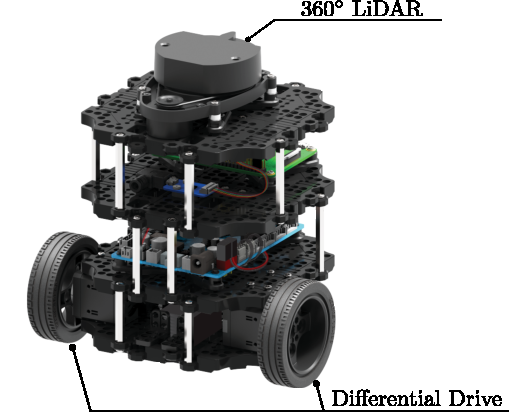
\includegraphics[width=0.5\linewidth]{turtlebot3_burger_components.pdf}
    \caption[]{ROBOTIS' TurtleBot3 Burger platform, with a mounted 360$^\circ$ LiDAR on top, and a differential drive (image source: www.robosklep.com).}
    \label{fig:turtlebot3-burger}
\end{figure}
The mounted 2D LiDAR provides range and angle measurements from the environment with $360^\circ$ field of view.
This particular model (LDS-01) has an angular resolution of $1^\circ$, detection range of $0.12-3.5$ m-s, % ! TODO validate data
and accuracy (3$\sigma$) of $\pm$15 mm-s (actually the precision is distance dependent, but this effect is not considered).
Invalid readings indicate out of range measurements. One full measurement is shown in Figure~\ref{fig:lidar-readings}.
\begin{figure}[htbp]
    \centering
    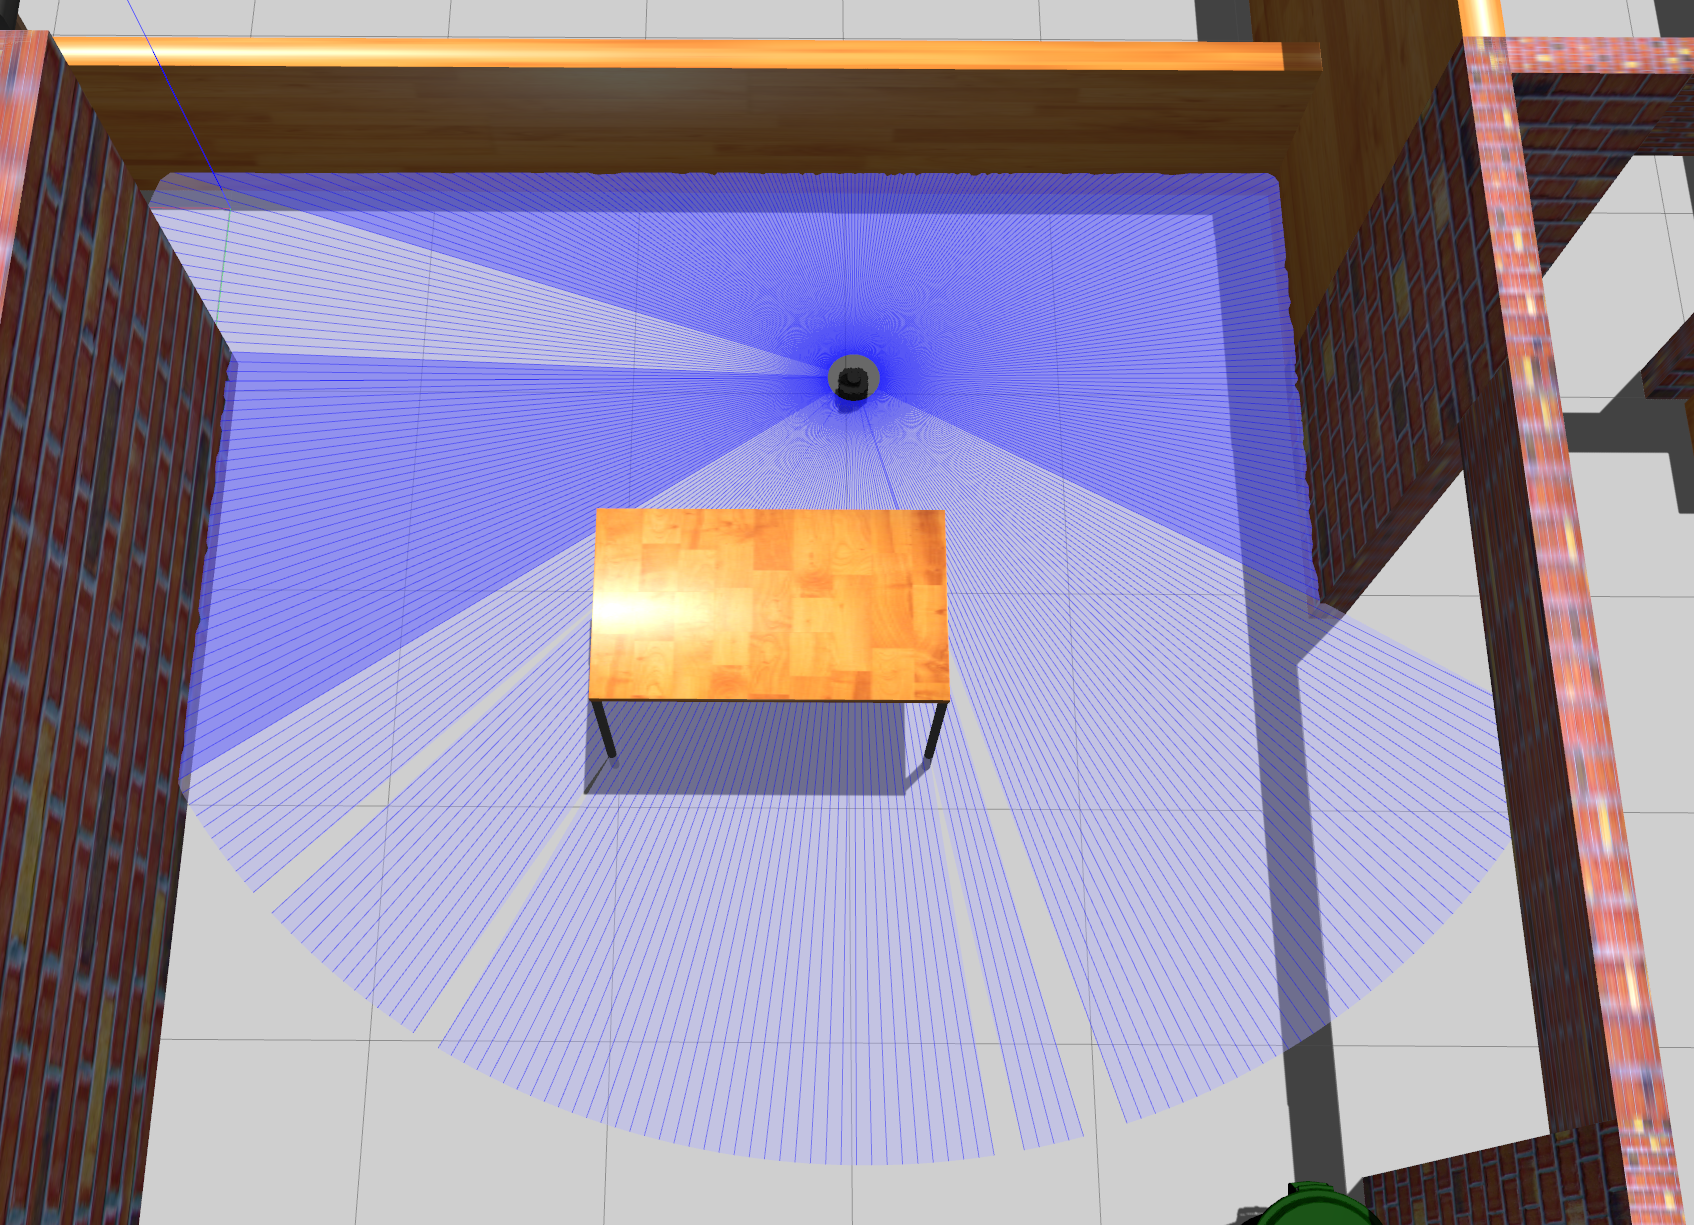
\includegraphics[width=0.6\linewidth]{lidar-visu.png}
    \caption{Visualized 2D LiDAR measurement of the TurtleBot3 in a house environment, using the Gazebo simulator.}
    \label{fig:lidar-readings}
\end{figure}

The platform has 2 independently-driven wheels, and one free turning wheel, which
makes it eligible to be modelled by differential drive kinematics.
The odometry is conducted by (simulated) rotary encoder readings from the two wheels separately.
Originally the out-of-the-box ROS-Gazebo model by ROBOTIS did not considered odometry noise,
which had to be manually added in order to efficiently model real world conditions.
Precisely modelling odometry error is a difficult task, and even nowadays is an actively researched topic \cite{Fazekas2021}.
However, this degree of precision is not required here.
Instead, both encoder readings are simply corrupted by a random variable each  ($\xi_L$ for the left wheel, $\xi_R$ for the right), obtained as
\begin{align}
    \xi_L \sim \mathcal{N}(0,\alpha v_L^{2}), \\
    \xi_R \sim \mathcal{N}(0,\alpha v_R^{2}),
\end{align}
where $\mathcal{N}(\mu,\sigma^{2})$ stands for a normal distribution with mean $\mu$ and variance $\sigma^{2}$,
$\alpha$ is a scaling parameter, and $v_L, v_R$ are the corresponding velocities. Applying this small modification,
ROS provides noisy odometry data at each tilmestep, which then can be used to establish the motion model of the robot (see Subsection~\ref{subsec:mot-model}).

\subsection{The Map}
The environment of the agent is represented by a 2D Occupancy Grid Map (OGM) \cite{Moravec1985}.
This model describes the environment by dividing it to finitely many grid cells, where each grid cell is a random binary variable,
representing that whether it’s occupied, or not.
Upon creating the OGM, the occupancy value of each cell (the probability, that its occupied) is iteratively updated.
To obtain a final map, these values are thresholded, producing values of 1 if the cell is \emph{mostly} occupied,
or 0 is its \emph{mostly not}.
The top-down view of the TurtleBot3 House by ROBOTIS and the corresponding OGM can be seen in Figure~\ref{fig:tb3-house-ogm},
which was obtained by the SLAM GMapping algorithm~\cite{Grisetti2007}.
For a pure localization task, the map is considered as ground truth,
therefore the previously introduced odometry noise was omitted during the mapping process.
\begin{figure}[htbp]
    \centering
    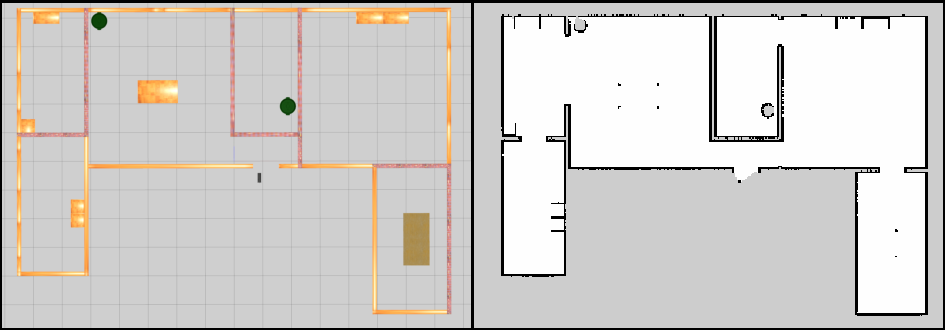
\includegraphics[width=\linewidth]{tb3-house-ogm.pdf}
    \caption{The top-down view of the TurtleBot3 House in Gazebo, and its OGM representation (mind the open doors in the building).
        Grey pixels represent unknown area, black pixels are occupied, white pixels are free cells.
        1 pixel (cell) in the OGM has a size of $0.05 \times 0.05$ m. }
    \label{fig:tb3-house-ogm}
\end{figure}
\subsection{The Motion Model}\label{subsec:mot-model}
Now that the hardware and the underlying localization task is introduced, the two main parts of the
Bayesian recursion is going to be described in the following subsections: the motion model, and the measurement model.

The motion model is used to describe the probability distribution of
$p(\mathbf{x}_t | \mathbf{x}_{t-1},\mathbf{u}_t)$. \linebreak
Without any external information, the pose of the robot at time $t$ can be estimated based on the previous pose
at time $t-1$, and the control input at time $t$. Naturally, this estimation will be disrupted by tire slippage and drift.
Due to the incremental nature, these errors are integrated over time, thus making the estimation more and more
uncertain.

The motion model describes this transition using the kinematic model of the agent.
Based on the inputs, two distinct probabilistic models can be established, introduced in \cite{Thrun2005}: the velocity motion model,
and the odometry motion model. Here, only the latter is detailed.

If the odometry of the robot is available (i.e. by integrating wheel encoder measurements),
they can be treated as a control input:
\begin{equation}
    \mathbf{u}_t = (\overline{\mathbf{x}}_t\;\;\overline{\mathbf{x}}_{t-1})^\top =
    \left(\overline{x}_t\;\;\overline{y}_t\;\;\overline{\theta}_t\;\;\overline{x}_{t-1}\;\;\overline{y}_{t-1}\;\;\overline{\theta}_{t-1}\right)^\top.
\end{equation}
The key is the fact that the relative difference between
two consecutive odometry data is a good estimation of the relative difference between
the two consecutive true poses, if the timestep is sufficiently small.

The transition between the state $\mathbf{x}_{t-1}$ and $\mathbf{x}_{t}$ is simplified as a sequence of a rotation, a translation,
and another rotation.
These are indicated in Figure~\ref{fig:odom-mot-model}. with $\delta_{\mathrm{rot1}}$, $\delta_{\mathrm{trans}}$,
and $\delta_{\mathrm{rot2}}$ respectively.
It's important to mention that this separation to rotational and translational components is arbitrary
(introduced by Thrun et al. in~\cite{Thrun2005}); for another approach, see~\cite{Eliazar2004}.
\begin{figure}[htbp]
    \centering
    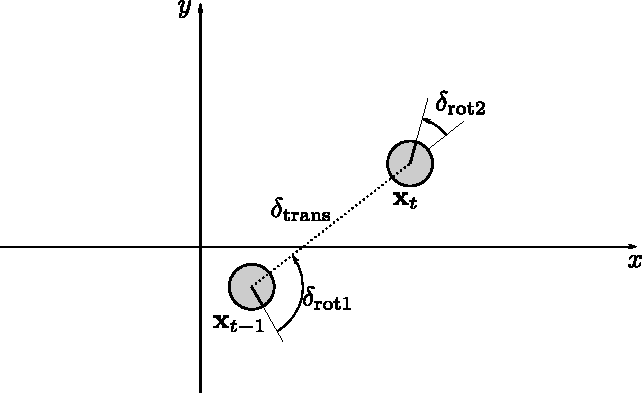
\includegraphics{odometry-motmodel.pdf}
    \caption{The rotation-translation-rotation transition sequence from state $\mathbf{x}_{t-1}$ to $\mathbf{x}_{t}$.}
    \label{fig:odom-mot-model}
\end{figure}

The control input $\mathbf{u}_t$
then transformed to the three transition components as:
\begin{align}
    \delta_{\mathrm{rot} 1} & =\arctan\!2\left(\overline{y}_{t}-\overline{y}_{t-1}, \overline{x}_{t}-\overline{x}_{t-1}\right)-\overline{\theta}_{t-1}, \\
    \delta_{\text {trans }} & =\sqrt{\left(\overline{x}_{t-1}-\overline{x}_{t}\right)^{2}+\left(\overline{y}_{t-1}-\overline{y}_{t}\right)^{2}},        \\
    \delta_{\mathrm{rot} 2} & =\overline{\theta}_{t}-\overline{\theta}_{t-1}-\delta_{\mathrm{rot} 1}.
\end{align}
To model odometry noise, the inputs are treated as random variables, formulated by
\begin{align}
    \hat{\delta}_{\mathrm{rot} 1} & = \delta_{\mathrm{rot} 1} + \xi_{\mathrm{rot1}},
    \quad                         & \xi_{\mathrm{rot1}} \sim \mathcal{N}(0,\alpha_1\delta_{\mathrm{rot1}}^2+\alpha_2\delta_{\mathrm{trans}}^2),                             \\
    \hat{\delta}_{\text {trans }} & = \delta_{\mathrm{trans}} + \xi_{\mathrm{trans}},
    \quad                         & \xi_{\mathrm{trans}} \sim \mathcal{N}(0,\alpha_3\delta_{\mathrm{trans}}^2+\alpha_4(\delta_{\mathrm{rot1}}^2+\delta_{\mathrm{rot2}}^2)), \\
    \hat{\delta}_{\mathrm{rot} 2} & = \delta_{\mathrm{rot} 2} + \xi_{\mathrm{rot2}},
    \quad                         & \xi_{\mathrm{rot2}} \sim \mathcal{N}(0,\alpha_1\delta_{\mathrm{rot2}}^2+\alpha_2\delta_{\mathrm{trans}}^2),
\end{align}
where $\alpha_1,\alpha_2,\alpha_3,\alpha_4$ are error parameters.

Then, using the control inputs and the previous state, samples from $p(\mathbf{x}_t | \mathbf{x}_{t-1},\mathbf{u}_t)$
are obtained by,
\begin{align}
    x_t          & = x_{t-1} + \hat{\delta}_{\mathrm{trans}}\cos(\theta + \hat{\delta}_{\mathrm{rot1}}), \\
    y_t          & = y_{t-1} + \hat{\delta}_{\mathrm{trans}}\sin(\theta + \hat{\delta}_{\mathrm{rot1}}), \\
    \theta_t     & = \theta_{t-1} + \hat{\delta}_{\mathrm{rot1}} + \hat{\delta}_{\mathrm{rot2}},         \\
    \mathbf{x}_t & = \left(x_t\;\;y_t\;\;\theta_t\right)^\top.
\end{align}

\section{Measurement Model}

\subsection{Introduction}
As the form of the motion model depends on many factors, for example the kinematics of the robot
(differential drive, car like structure, etc.), and the used control input interpretation
(odometry-based, or velocity-based), measurement models are no different.
However, the used proprioceptive sensor (LiDAR), and the map representation (OGM) in this task
narrow the possibilities.

\subsection{Standard Measurement Models on Different Map Realizations}
Wide-spread algorithms are often established for topological (feature-based) maps.
Here, the environment is described by detected shapes (features), rather than using a location based representation
like the OGMs do, as they assign an occupancy value for every location on the map.

For a topological map, the probability distribution of $p(\mathbf{\mathbf{z}}_t | \mathbf{x}_t)$,
enhanced with the known map $\mathbf{m}$ (resulting in $p(\mathbf{\mathbf{z}}_t | \mathbf{x}_t,\mathbf{m})$)
is described a Gaussian distribution:
\begin{align}
    h(\mathbf{x}_t,\mathbf{m}) = \mathbf{z}^*_t + \xi, \quad \xi \sim \mathcal{N}(0,\mathbf{R}), \\
    \Rightarrow p(\mathbf{\mathbf{z}}_t | \mathbf{x}_t,\mathbf{m}) \sim \mathcal{N}(\mathbf{z}_t^*,\mathbf{R}).
\end{align}
where $\mathbf{R}$ is the covariance matrix of the measurement.
This closed-form description is required for Kalman Filters.

However, for location based (metric) maps, the form of $\mathbf{m}$ is different, therefore
to make the above model work, features have to be extracted \cite{Durrant-Whyte1991},
effectively making the map feature-based.

For purely metric maps (without feature extraction), Thrun et al. proposed the \emph{beam range finder model}
in \cite{Thrun2005}, especially fitted for range finders, like LiDARs, or sonars.
This model describes  $p(\mathbf{\mathbf{z}}_t | \mathbf{x}_t,\mathbf{m})$ as a composition of
probability densities, resulting in a distribution indicated in Figure \ref{fig:beam-model}.
Here, the value $\mathbf{z}_t^*$ is calculated by ray tracing: at a given robot pose,
the expected measurement can be calculated, by tracing a ray along the map, starting form
the robot pose, and ending in the nearest obstacle. Then the travelled distance is recorded,
which together with the angle of the beam, serves as $\mathbf{z}_t^*$.

The resulting distribution combines different measurement error possibilities:
random measurements (uniform distribution), local measurement noise (Gaussian distr.),
failures (``very narrow'' uniform distribution, modelling a Dirac delta) and unexpected
objects (exponential distribution).
\begin{figure}[htbp]
    \centering
    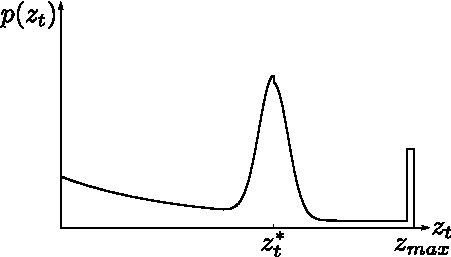
\includegraphics{beam-model.pdf}
    \caption{The probability distribution of $p(z_t | \mathbf{x}_t,\mathbf{m})$.
        The figure is based on \cite{Thrun2005}.}
    \label{fig:beam-model}
\end{figure}

However, the resulting probability distribution does not have a closed form description, which is
not a problem for particle filters, but it is for Kalman filters.

\subsection{The Distance Function based Measurement Model}
The method, which enables the use of Kalman filters with laser range finder measurements on an OGM is proposed
by Dantanarayana et al. in \cite{Dantanarayana2013,Dantanarayana2016}.
In the following, this method is going to be detailed, based on \cite{Dantanarayana2016b}.

The key idea is the utilization of the distance transform (DT), which is widely used in
image processing.
For a given binary image (or in this case, an OGM), the distance transform
produces an image/map (with the same size), where the value of each pixel/cell is
determined by the closest distance to any occupied pixel/cell.
If $V$ is the set of the occupied cells, and $\mathbf{x}$ is an arbitrary point on the map, then
\begin{equation}
    d_{D F}=D F(\mathbf{x})=\min _{\mathbf{v}_{\mathbf{j}} \in V}\left\|\mathbf{x}-\mathbf{v}_{\mathbf{j}}\right\|,
\end{equation}
in which an Euclidean norm is usually applied.
The distance transform then could be pre-calculated for a given map.
Figure \ref{fig:simple-dt} shows the DT in a simplified environment,
while the DT of one part of the OGM from Figure \ref{fig:gazebo-map-ogm-dt}. can be seen on Figure
\begin{figure}[htbp]
    \centering
    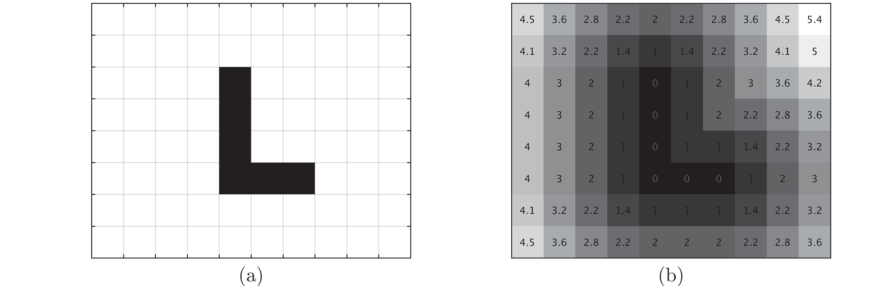
\includegraphics{simple_dt.pdf}
    \caption{A simple shape and its distance transform. Figure source: \cite{Dantanarayana2016b}.}
    \label{fig:simple-dt}
\end{figure}
\begin{figure}[htbp]
    \centering
    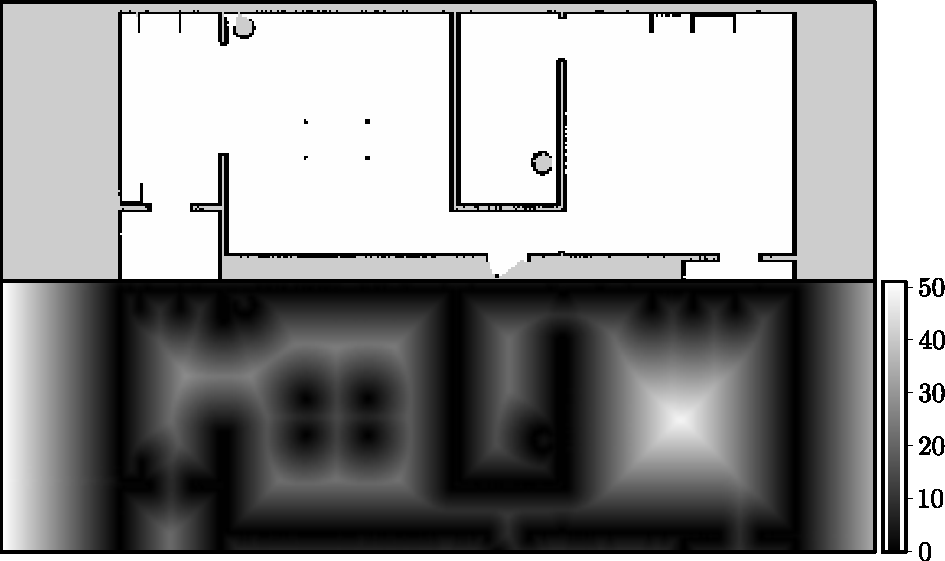
\includegraphics{dt_on_ogm.pdf}
    \caption{Part of the OGM of the TurtleBot3 House, and its distance transform.}
    \label{fig:gazebo-map-ogm-dt}
\end{figure}

Now using the LiDAR measurements, which in this case come in the form of angle-range pairs,
each detection can be transformed to map coordinates, and assigned a distance transform value.
Theoretically, if the estimated pose of the robot, and the true pose of the robot aligns,
and the sensor is noiseless, each reading should indicate an occupied cell on the OGM.
Therefore, all the projected detections should have a DT of zero.
It other cases, the ray endpoints could end up on free cells, thus having a DT value larger,
than zero.

The method of transforming (projecting) the laser scans to the map, based on the estimated
location of the robot is shown in Figure \ref{fig:ogm-laser-projection}.
Mathematically, these projections are obtained as
\begin{equation}
    \mathbf{x}_{\mathrm{o}i} = \begin{bmatrix}x_{\mathrm{o}i}\\y_{\mathrm{o}i}\end{bmatrix}
    = \begin{bmatrix}x + r_i\cos(\varphi_i + \theta)\\y + r_i\sin(\varphi_i + \theta)\end{bmatrix},
\end{equation}
where the variables are according to Figure \ref{fig:ogm-laser-projection}. (the time dependency is omitted).
\begin{figure}[htbp]
    \centering
    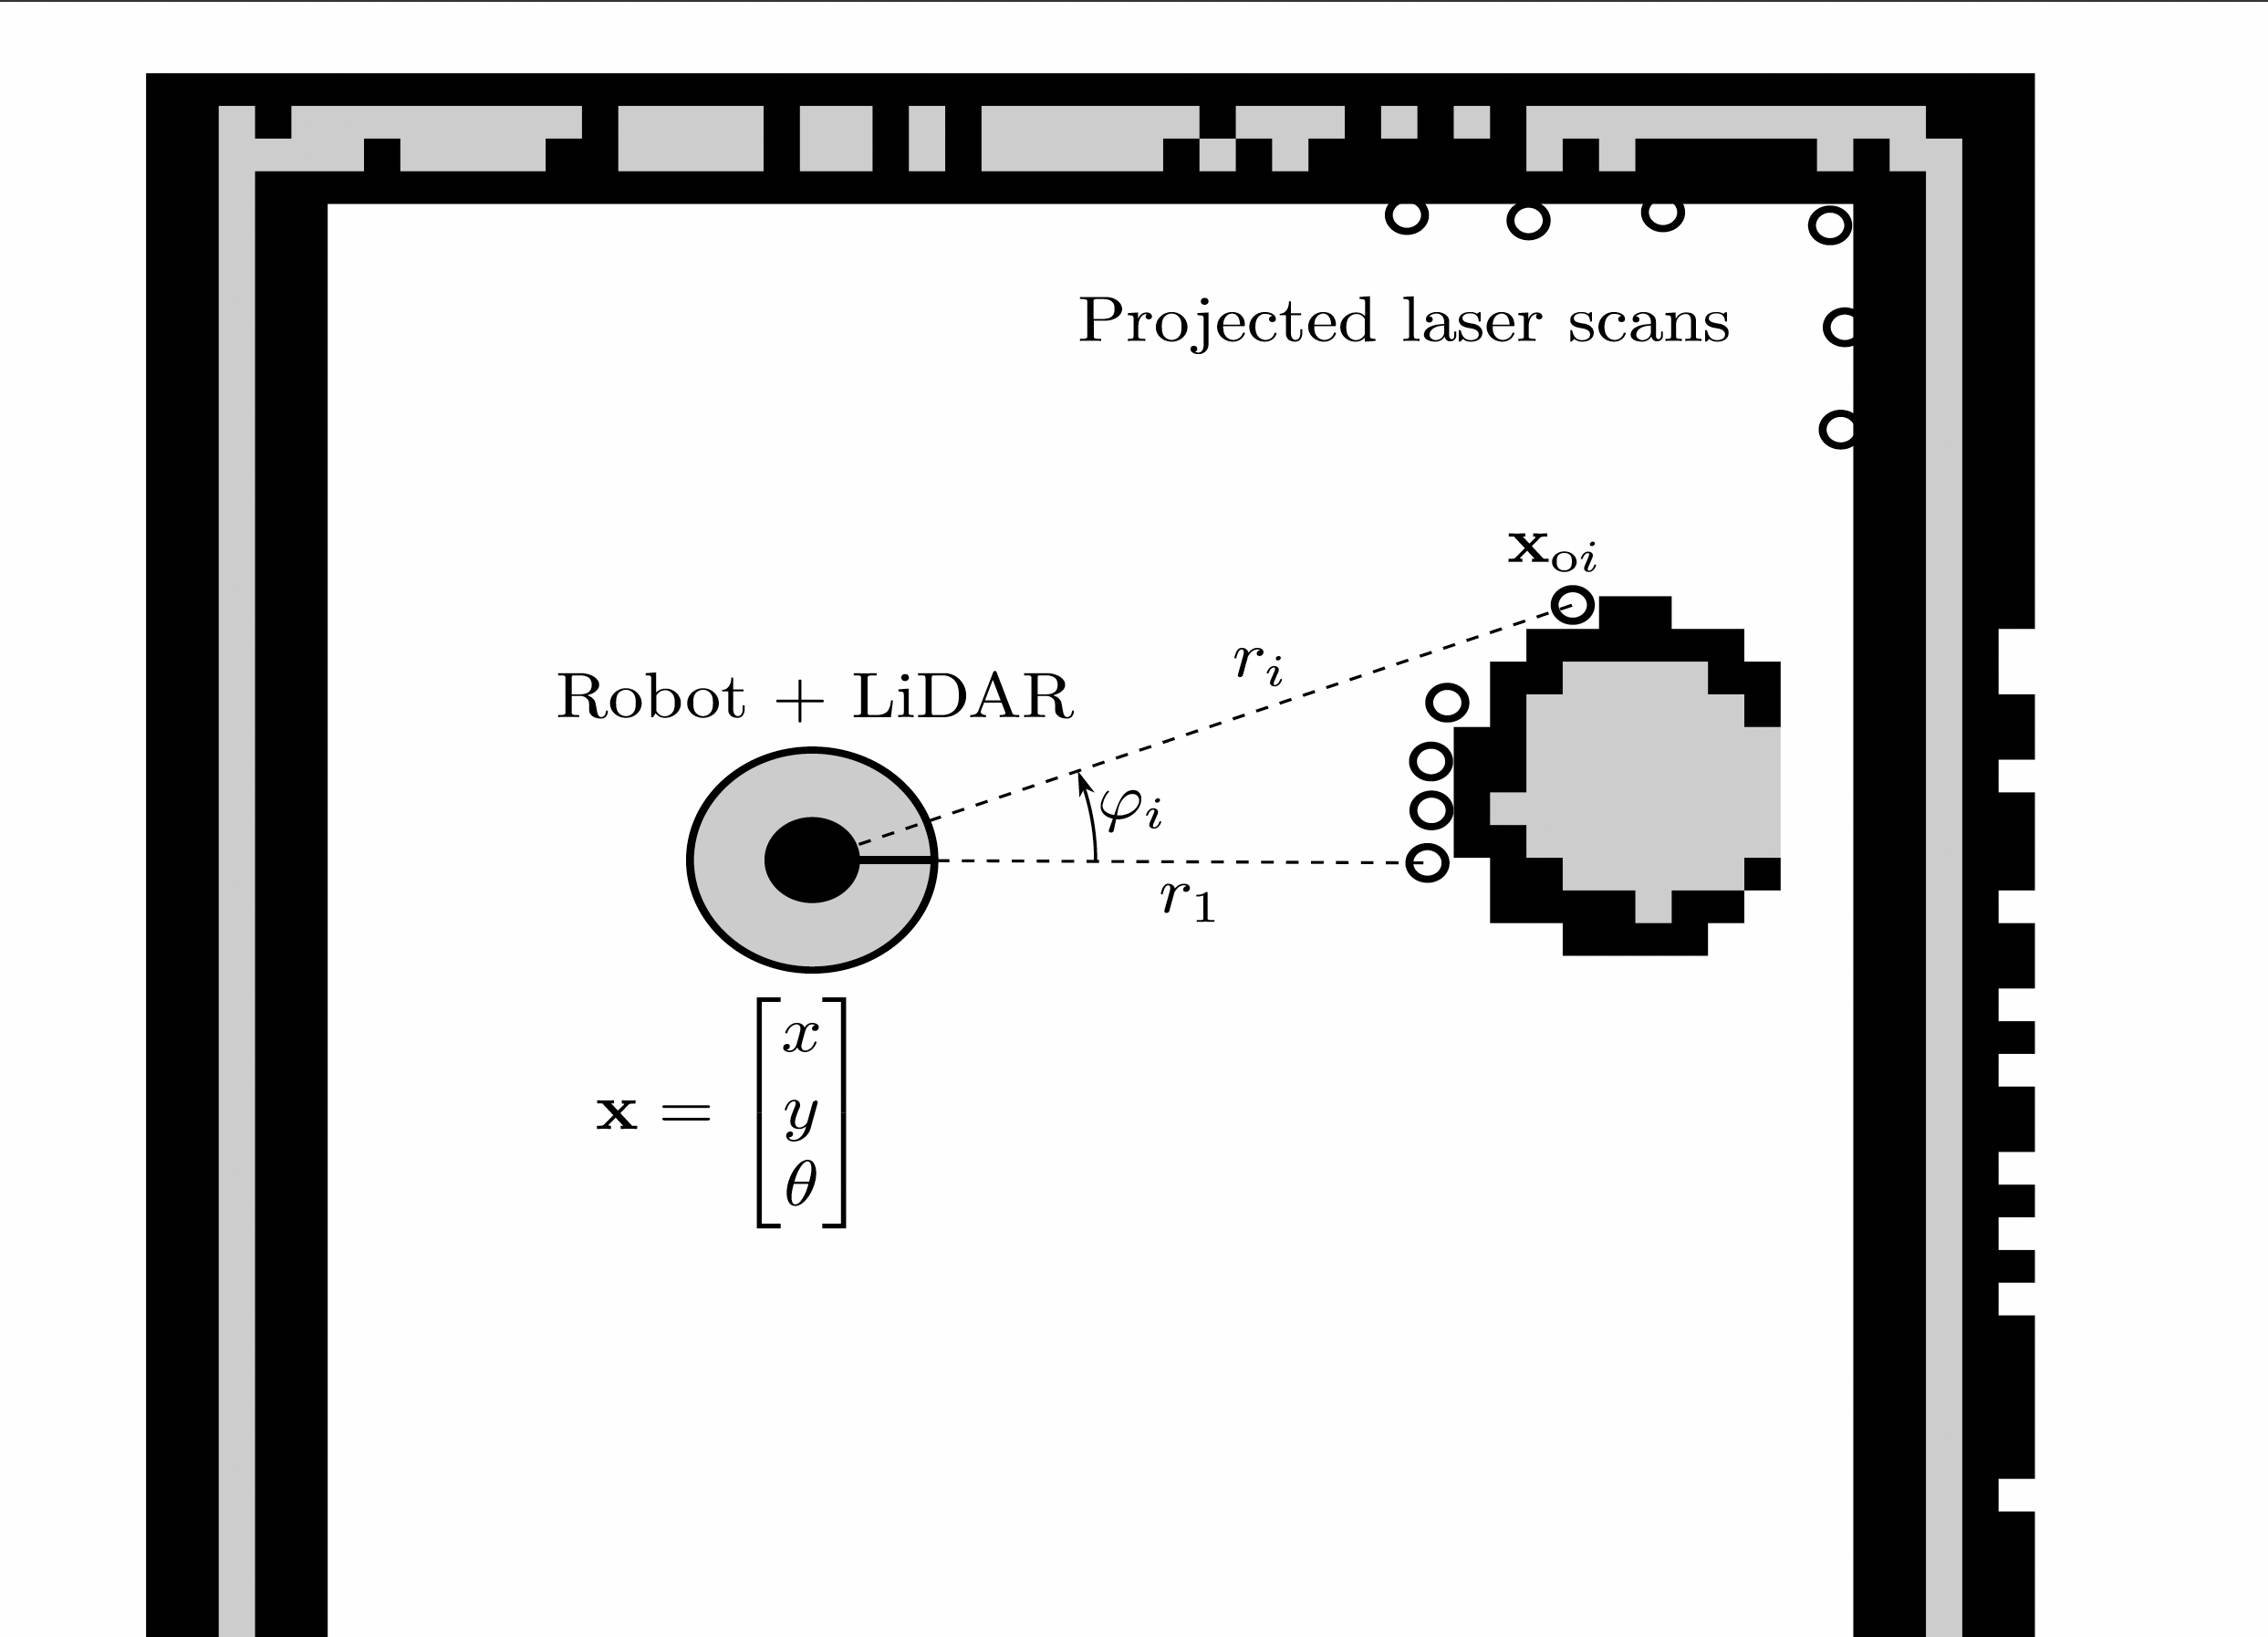
\includegraphics[width=0.95\linewidth]{dt_mapping_lidar}
    \caption{Projection of the LiDAR scans to the OGM, based on the pose of the robot.}
    \label{fig:ogm-laser-projection}
\end{figure}

Based on a set of measurements (for a whole revolution of the LiDAR), a vector can be constructed as follows:
\begin{equation}\label{eq:df-vector}
    \mathbf{d}_{\text{DF}} =
    \begin{bmatrix}
        DF(\mathbf{x}_{\text{o}1}) \\
        DF(\mathbf{x}_{\text{o}2}) \\
        \vdots                     \\
        DF(\mathbf{x}_{\text{o}n}) \\
    \end{bmatrix},
\end{equation}
where $n$ is the number of valid LiDAR readings for a whole revolution
(a valid reading occurs when the laser ray actually collided with an object within range, and this was
detected by the sensor).
To obtain a single scalar value, which indicates the disparity between the projected measurements,
and the map, the Chamfer distance (CD) is formulated. For a set of measurements,
\begin{equation}
    d_{\text{CD}} = \frac{1}{n}\sum_{i=1}^nDF(\mathbf{x}_{\text{o}i}).
\end{equation}
The CD is a good indicator for the estimation of the robot's pose: $CD=0$ means,
that every ray endpoint for a set of measurement at time $t$ is at the right place,
therefore the initial robot pose estimation is good.
Although, it is important to mention that this assumption does not hold in every
scenario. Consider an extreme case: for a whole revolution, the LiDAR only records
one measurement (one ray), and the OGM only contains many occupied cell.
Then the CD (effectively the DT) would equals to zero at a plethora of robot poses, thus not indicating the sought true pose.
For a detailed map and sufficiently many LiDAR reading per revolution, this deficiency is minimized.

Using the CD, the measurement model is formulated as
\begin{equation}
    p(\mathbf{\mathbf{z}}_t | \mathbf{x}_t, DF_t) \sim \mathcal{F}(d_{\text{CD}t},\boldsymbol\Sigma_{\text{CDt}}).
\end{equation},
where $\mathcal{F}$ denotes the folded Gaussian distribution.
The covariance is calculated as
\begin{equation}
    \boldsymbol\Sigma_{\text{CD}} = \mathbf{J}_{\text{CD}}\mathbf{R}\mathbf{J}_{\text{CD}}^{\top},
\end{equation}
where $\mathbf{R}$ is the measurement covariance matrix, and $\mathbf{J}_{CD}$ is the Jacobian of the
Chamfer distance with respect to $\mathbf{z}_i = \begin{bmatrix}\varphi_i&r_i\end{bmatrix}^{\top}$,
evaluated at $\mathbf{x}$. However, due to the assumption, that the measurement only has error
in $r_i$, the differentiation with regarding to $\varphi_i$ is omitted.

Due to the fact, that the expected CD is zero at the true pose,
the measurement equation has the close form of
\begin{equation}
    d_{CD} :=h(\mathbf{x}_t,\mathbf{z}_t) = 0,
\end{equation}
forming an implicit equation for $\mathbf{x}_t$ and $\mathbf{z}_t$, which is
applicable for Kalman filters.

\subsection{The Kalman Filters}
\subsubsection{Kalman Filter}
The Kalman filter (KF) assumes that ``everything'' \emph{is} linear and Gaussian, and under these assumptions it can be proved that ``everything'' \emph{stays} linear and Gaussian during the Bayes filter updates. A Gaussian distribution can be fully characterized by its first two moments, therefore the Kalman filter offers a recursion to calculate the mean $\boldsymbol{\mu}_t$ and the covariance $\mathbf{\Sigma}_t$ of the belief $bel(\mathbf{x}_t)$. In this context only the discrete-time KF is going to be discussed.

Consider the discrete-time (linear) state space model of a system:
\begin{align}\label{key}
    \mathbf{x}_t & = \mathbf{A}_t\mathbf{x}_{t-1} + \mathbf{B}_t\mathbf{u}_t + \mathbf{G}_t\mathbf{v}_t, \\
    \mathbf{z}_t & = \mathbf{C}_t\mathbf{x}_t + \mathbf{w}_t,
\end{align}
where $\mathbf{A}_t$ is the state transition matrix, $\mathbf{B}_t$ is the input gain, $\mathbf{G}_t$ is the noise gain, $\mathbf{C}_t$ is the measurement matrix. To incorporate uncertainties and inaccuracies into the system, the process noise $\mathbf{v}_t$ and the measurement noise $\mathbf{w}_t$ is introduced. Both are Gaussian random variables: $\mathbf{v}_t \sim \mathcal{N}(\mathbf{0},\mathbf{Q})$, $\mathbf{w}_t \sim \mathcal{N}(\mathbf{0},\mathbf{R})$, with $\mathbf{Q}$ as process noise covariance, and $\mathbf{R}$ as measurement noise covariance.

Using the linear nature of the model, and assuming, that the probability distributions in the Bayes filter are Gaussian distributions, the motion model has the following form:
\begin{equation}\label{key}
    p(\mathbf{x}_t|\mathbf{x}_{t-1}, \mathbf{u}_t) = \mathrm{det}(2\pi{\tilde{\mathbf{Q}}_t})^{-\frac{1}{2}}\mathrm{exp}\{-\frac{1}{2}(\mathbf{x}_t-\mathbf{A}_t\mathbf{x}_{t-1}-\mathbf{B}_t\mathbf{u}_t)^\top\tilde{\mathbf{Q}}_t^{-1}(\mathbf{x}_t-\mathbf{A}_t\mathbf{x}_{t-1}-\mathbf{B}_t\mathbf{u}_t)\},
\end{equation}
where $\tilde{\mathbf{Q}}_t = \mathbf{G}_t\mathbf{Q}_t\mathbf{G}_t^\top$.
The measurement model can be calculated similarly.

The derivation of the Kalman filter algorithm is not trivial, and does not fall within the scope of this document. The algorithm can be seen in Algorithm \ref{alg:kf}., where $\mathbf{I}$ denotes the identity matrix.

\begin{algorithm}
    \caption{Kalman filter($\boldsymbol{\mu}_{t-1},\mathbf{\Sigma}_{t-1},\mathbf{u}_t,\mathbf{z}_t$)}\label{alg:kf}
    \begin{algorithmic}[1]
        \BState \emph{prediction}:
        \State\indent$\overline{\boldsymbol{\mu}}_t = \mathbf{A}_t{\boldsymbol{\mu}}_{t-1} + \mathbf{B}_t\mathbf{u}_t$
        \State\indent $\overline{\mathbf{\Sigma}}_t = \mathbf{A}_t\mathbf{\Sigma}_{t-1}\mathbf{A}^\top_t + \tilde{\mathbf{Q}}_t$
        \BState \emph{update/correction}:
        \State\indent $\mathbf{K}_t = \overline{\mathbf{\Sigma}}_t\mathbf{C}_t^\top\left(\mathbf{C}_t\overline{\mathbf{\Sigma}}_t\mathbf{C}_t^\top+\mathbf{R}_t\right)^{-1}$
        \State\indent $\boldsymbol{\mu}_t = \overline{\boldsymbol{\mu}}_t + \mathbf{K}_t\left(\mathbf{z}_t-\mathbf{C}_t\overline{\boldsymbol{\mu}}_t\right)$
        \State\indent $\mathbf{\Sigma}_t = \left(\mathbf{I}-\mathbf{K}_t\mathbf{C}_t\right)\overline{\mathbf{\Sigma}}_t$
        \State\Return $\boldsymbol{\mu}_t,\mathbf{\Sigma}_t$
    \end{algorithmic}
\end{algorithm}
\subsubsection{Extended Kalman Filter}
However, assuming a linear state space model is a rather strong assumption. For a nonlinear model the general state space equations are (not considering nonlinear noise gain):
\begin{align}\label{key}
    \mathbf{x}_t & = \mathbf{a}(\mathbf{u}_t,\mathbf{x}_{t-1}) + \mathbf{G}_t\mathbf{v}_t, \\
    \mathbf{z}_t & = \mathbf{h}(\mathbf{x}_t) + \mathbf{w}_t.
\end{align}
The state propagation function $\mathbf{a}(.)$ can be locally linearized around the previous state $\mathbf{x}_{t-1} = \boldsymbol{\mu}_{t-1}$, resulting $\tilde{\mathbf{A}}_t$. The measurement function $\mathbf{h}(.)$ is linearized around the current predicted state $\overline{\boldsymbol{\mu}}_t$, resulting $\mathbf{H}_t$.

The EKF algorithm is the extension of the KF by handling nonlinear state equations through their linearized forms. Algorithm \ref{alg:ekf}. contains the EKF algorithm.

\begin{algorithm}
    \caption{Extended Kalman filter($\boldsymbol{\mu}_{t-1},\mathbf{\Sigma}_{t-1},\mathbf{u}_t,\mathbf{z}_t$)}\label{alg:ekf}
    \begin{algorithmic}[1]
        \BState \emph{prediction}:
        \State\indent$\overline{\boldsymbol{\mu}}_t = a(\mathbf{u}_t,\boldsymbol{\mu}_{t-1})$
        \State\indent $\overline{\mathbf{\Sigma}}_t = \tilde{\mathbf{A}}_t\mathbf{\Sigma}_{t-1}\tilde{\mathbf{A}}^\top_t + \tilde{\mathbf{Q}}_t$
        \BState \emph{update/correction}:
        \State\indent $\mathbf{K}_t = \overline{\mathbf{\Sigma}}_t\mathbf{H}_t^\top\left(\mathbf{H}_t\overline{\mathbf{\Sigma}}_t\mathbf{H}_t^\top+\mathbf{R}_t\right)^{-1}$
        \State\indent $\boldsymbol{\mu}_t = \overline{\boldsymbol{\mu}}_t + \mathbf{K}_t\left(\mathbf{z}_t-h(\overline{\boldsymbol{\mu}}_t)\right)$
        \State\indent $\mathbf{\Sigma}_t = \left(\mathbf{I}-\mathbf{K}_t\mathbf{H}_t\right)\overline{\mathbf{\Sigma}}_t$
        \State\Return $\boldsymbol{\mu}_t,\mathbf{\Sigma}_t$
    \end{algorithmic}
\end{algorithm}
\subsubsection{Advantages and Disadvantages of Kalman Filters}

Under linear and Gaussian assumptions the Kalman filter yields the optimal estimation (by calculated mean square error). However, these criteria are rarely satisfied, and the optimal estimation property does not hold any more. Another major problem comes from the nature of Gaussian distributions: they are unimodal, therefore the Kalman Filter cannot track multiple high-probability hypotheses.

EKF offers one type of solution to the nonlinearity: linearization by Taylor expansion. This however, introduces linearization error into the system. For highly nonlinear equations not only the first order approximation is the problem, but its center point as well. As were mention before, the state equation is linearized around the previous state; but now this state also an approximation. This overall effect can cause the algorithm to diverge, or to yield poor results. In addition, the initial conditions also have to be carefully chosen in order to obtain desired results.

Despite these, the EKF is still one of the most popular state estimation algorithm in robotics, and often used in Global Navigation Satellite Systems (GNSS) as well, thanks to its computational simplicity and easy  implementation. Other Kalman filter based realizations are including but not limited to the unscented Kalman filter (UKF), which uses a different type of linearization instead of the Taylor expansion based one, and the ensemble Kalman Filter (EnKF), which is suited for high dimensional estimation problems.

\subsection{The Particle Filters}
\subsubsection{Main concepts}

Particle filters (PF) are used to solve nonlinear filtering problems. Unlike EKF and other nonlinear extensions of the Kalman filter, this method uses a nonparametric representation of the estimated posterior. This nonparametric nature enables the estimation of various distributions, including multimodal and/or non-Gaussian.

The main concept in PF is to represent arbitrary probability distributions by cumulative probability mass of particles. When for example a Gaussian distribution is sampled multiple times, more samples come from regions with high probability density. This (trivial) effect can also be used in reverse: if samples are given, what is the probability distribution from which they were sampled? If the number of particles is sufficiently large (ideally infinity), they can offer a good approximation of the probability distribution.

The Bayesian filtering framework is implemented in as follows . First, draw $N$ samples (called as particles) from a prior distribution. Then migrate each of these particles according to the motion model. Now the particle set will approximately describe the predicted belief \eqref{eq:predbel}. (In the KF this predicted belief was described by its mean and covariance, as it was assumed to be a Gaussian distribution. Now, it is described by particles, and the Gaussian nature is not required.)

The KF used the $\mathbf{K}_t$ Kalman gain as a weight to calculate the posterior from the predicted belief. Particle filters use \emph{importance sampling} for this task: each sample is given an importance weight which describes its relevance. If this relevance is high, it means that the specific particle is a good approximation of the true (sought) state. Choosing a proper weighting method is a difficult task. Generally, weights are calculated from a target and a proposal distribution. The target distribution is the posterior, the proposal distribution however, can be arbitrary (under some criteria). Now using the particles and their weights, the posterior distribution is approximated.

The next step of the filter is optional, although essential: resampling. Here, a new (same sized) particle set is constructed by drawing particles from the old set with replacement, according to their weights. This means that some  particles can be chosen multiple times (more likely high-weighted ones), thus certain particles can be eliminated. Finally, their weights are equalized. With the resulting particle set (either the new, redrawn one, or the old, weighted one), the algorithm is repeated in the new time step.

Generally, the most demanding task when designing PFs is the proper selection of the proposal density and the resampling frequency (i.e. when to resample). Choosing the right proposal distribution and the right time to resample is crucial in the performance of the PF. In the next subsection, the bootstrap particle filter method with adaptive resampling is introduced in detail.
\subsubsection{The Bootstrap Particle Filter}

Denote the particles and their set at time $t$  as:
\begin{equation}\label{key}
    \mathcal{X}_t = \{\mathbf{x}_t^{[1]},\mathbf{x}_t^{[2]}, \dots \mathbf{x}_t^{[N]}\}.
\end{equation}

The bootstrap particle filter uses the predicted belief as the proposal distribution, which results in the following weight assignment:
\begin{equation}\label{key}
    w_t^{[n]} = p(\mathbf{z}_t|\mathbf{x}_t^{[n]}).
\end{equation}
This means, that  if the proposal distribution is the predicted belief, the weight is calculated according to the measurement model (the mathematical derivation is omitted). In the original algorithm \cite{bpf}, resampling is performed in every step. However, this might not be beneficial, therefore an effective sample size based adaptive resampling is applied \cite{ess}. One major problem with particle filters is when many particles are in irrelevant locations, therefore only a few of them represent the high probability region of the posterior properly. This called particle degeneracy. However, the value of the weights can indicate this ill-favored situation. The effective sample size ($ESS$ or $N_{\mathrm{eff}}$) can be approximated as the following:
\begin{equation}\label{eq:neff}
    N_{\mathrm{eff}} = \frac{1}{\sum_{i = 1}^{N}(w_t^{[i]})^2},
\end{equation}
if the sum of weights are 1 (normalized). Consider the situation where all the weights are equal, thus $w_t^{[1]} = w_t^{[2]} = \dots = w_t^{[N]} = 1/N$. This results in $N_{\mathrm{eff}} = N$, which is beneficial. The worst case scenario is when one weight is 1, and all the others are 0, which results in $N_{\mathrm{eff}} = 1$. It is common to define a threshold $N_{T}$, where if $N_{\mathrm{eff}} < N_T$, a resampling is performed.

The pseudocode of the bootstrap particle filter with adaptive resampling is presented in Algorithm \ref{alg:bpf}.
\begin{algorithm}[b!]
    \caption{Bootstrap particle filter ($\mathcal{X}_{t-1}, \mathbf{u}_t, \mathbf{z}_t$)}\label{alg:bpf}
    \begin{algorithmic}[1]
        \State $\overline{\mathcal{X}}_t = \mathcal{X}_t = \emptyset$
        \For{ $n$ = 1 to $N$ }
        \State sample $\mathbf{x}_t^{[n]} \sim p(\mathbf{x}_t|\mathbf{x}_{t-1}^{[n]},\mathbf{u}_t)$
        \State$w_t^{[n]} = p(\mathbf{z}_t|\mathbf{x}_{t}^{[n]})w_{t-1}^{[n]}$
        \EndFor
        \State calculate weight sum $\hat{w}_{t} = \sum_{i = 1}^{N}w_t^{[i]}$
        \For{ $n$ = 1 to $N$ }
        \State normalize $w_t^{[n]} = w_t^{[n]}\hat{w}_t^{-1}$
        \State$\overline{\mathcal{X}}_t = \overline{\mathcal{X}}_t + \langle \mathbf{x}_t^{[n]},w_t^{[n]}\rangle$
        \EndFor
        \State calculate $N_{\mathrm{eff}}$ using \eqref{eq:neff}
        \If{$N_{\mathrm{eff}} < N_T$}
        \For{ $n$ = 1 to $N$ }
        \State draw $i$ with probability $\propto w_t^{[i]}$ \label{line:bpf_resaml}
        \State${\mathcal{X}}_t ={\mathcal{X}}_t + \langle \mathbf{x}_t^{[i]},N^{-1}\rangle$
        \EndFor
        \State\Return $\mathcal{X}_t$
        \Else
        \State$\mathcal{X}_t = \overline{\mathcal{X}}_t$
        \State\Return $\mathcal{X}_t$
        \EndIf
    \end{algorithmic}
\end{algorithm}
There are several ways to implement the resampling in Line \ref{line:bpf_resaml}: the most basic method is the ''roulette wheel'' sampling, but in this scenario, the stratified sampling \cite{stratified} is used.
\subsubsection{Advantages and Disadvantages of Particle Filters}\label{sec:pf_adv_disadv}
Particle filters are well suited for nonlinear and non-Gaussian state estimation. They are especially versatile: many PF variations can be constructed for a plethora of applications. They are easy to implement, and demand low computational power. Their main usages are most importantly robot localization \cite{amcl} and  SLAM \cite{gmapping1}.

However, its numeric solution method (approximate probability distributions by samples) leaves a lot of room for errors. Most importantly, the particle filter can suffer from the so called \emph{curse of dimensionality}, which is described in \cite{bpf} as ``One must expect $N$ (the number of particles) to rise rapidly with the dimension of the space (...) It is most difficult to make any precise provable statement on the crucial question of how many samples are required to give a satisfactory representation of the densities for filter operation''. With a good proposal distribution, this unwanted property can be avoided. Daum and Huang in \cite{curse_of_dim} showed that the BPF suffers from this phenomena, while for example the unscented particle filter does not.

The curse of dimensionality problem is connected to the so called particle degeneracy phenomenon. It means that only a low amount of samples estimates the target posterior efficiently; others are in regions with very low probability. This occurs when the proposal distribution and the target distribution are not matched well. Figure \ref{fig:pf-degen}. shows a setup which demonstrates this effect: the prior distribution (the predicted belief in the case of the BPF) is colored in blue, and represented by its particles, shown as black dots. The weighting of the particles is done according to the likelihood (red curve), which is the measurement model in the BPF. As a result, only 3 particles are going to have weights other, than 0. Upon resampling, only these 3 particles will represent the target posterior; the others are eliminated. (Of course the size of the particle set will not change, only that they are distributed across 3 distinct positions). By common sense, a probability distribution is hardly represented properly by 3 particles. Counter-intuitively, having a more precise sensor (i.e. having a ''thinner'' likelihood function) only makes this worse.

\begin{figure}[htb!]
    \centering
    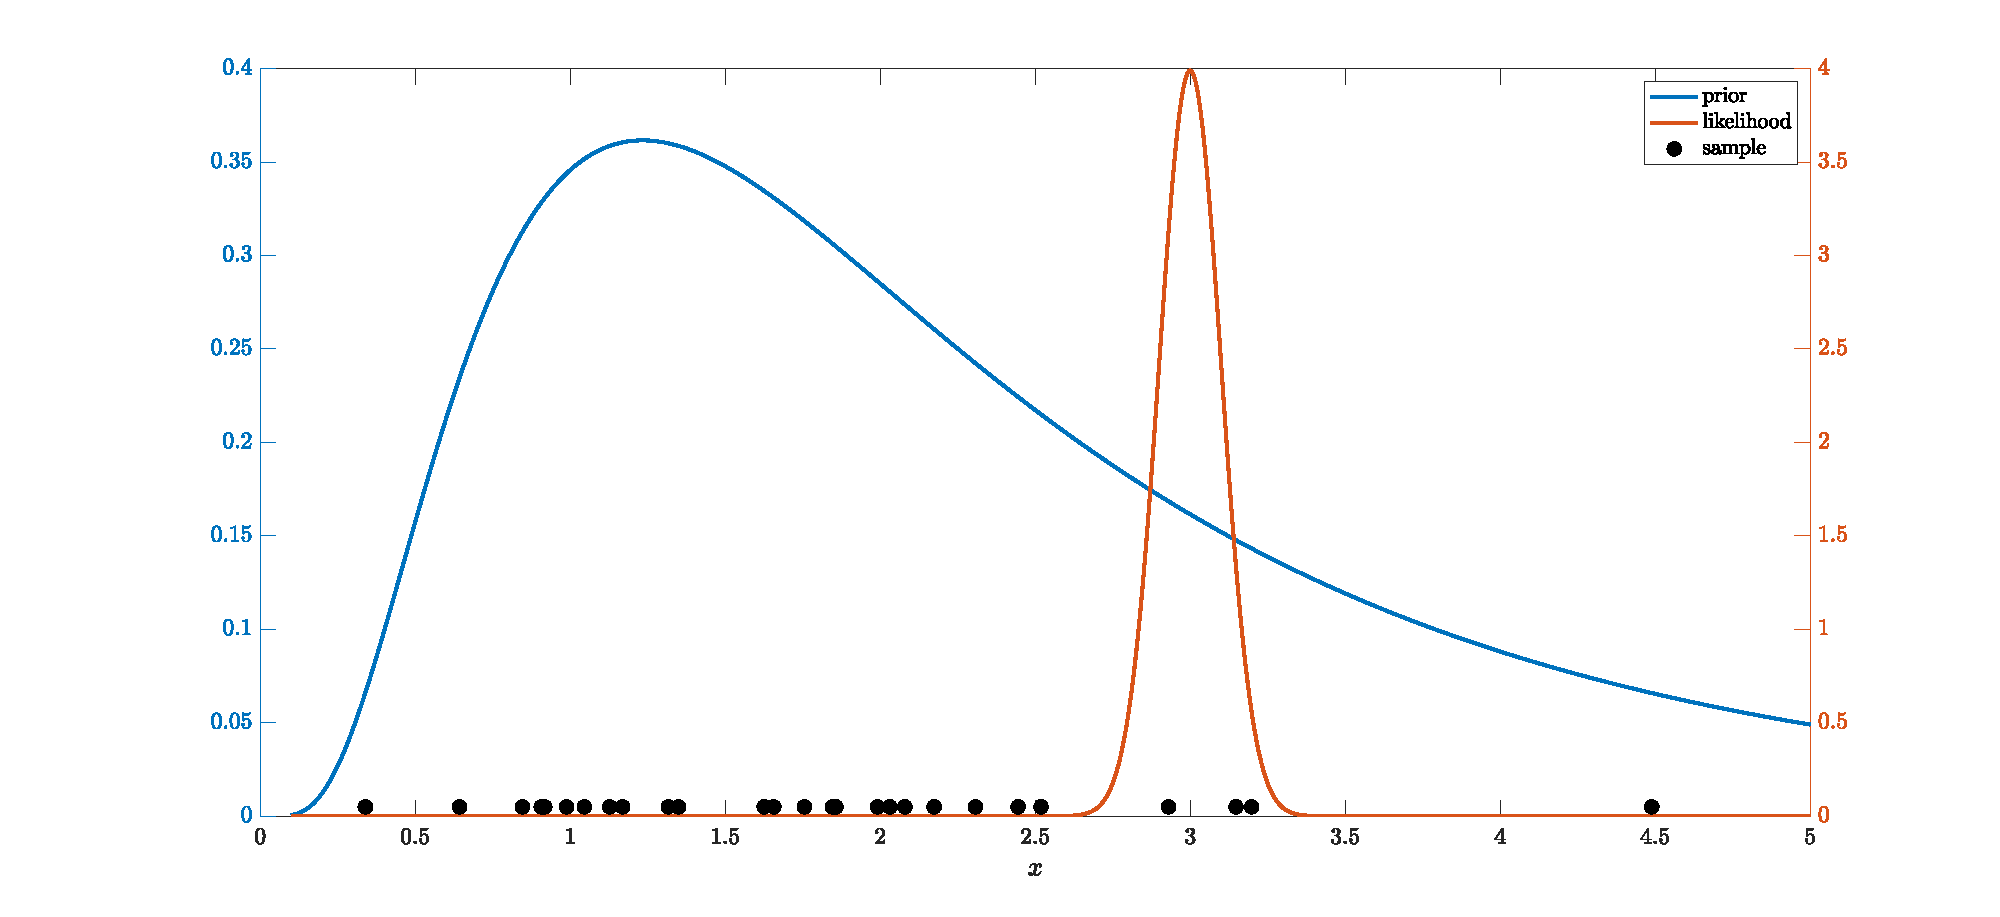
\includegraphics[width = \linewidth]{pf_degen.pdf}
    \caption{Particle degeneracy, shown in a one-dimensional example with 30 particles.}
    \label{fig:pf-degen}
\end{figure}
There are three possible ways to minimalize particle degeneracy: the most obvious one is to have more particles (populate the state space more densely). However, in higher dimensions this demands exponentially more particles. Another solution is to use a different proposal density, therefore having a different likelihood function. In this way the target distribution could be more effectively represented by particles. The third one is resampling: having more particles on top of each other in the same place is better than having only a few of them, while all the others are spread across the domain with negligible weights.


Although particle filters demand low computational power, this only holds when the algorithm is properly tuned, therefore requires the minimal amount of particles. A poor choice of a particle filter, or a poorly designed particle filter requires a lot of computational capacity to give proper results: the particle requirement can be in the order of millions. As were mentioned in \cite{curse_of_dim}, ``for typical low dimensional tracking problems, the PF requires 2 to 6 orders of magnitude more computer throughput than the extended Kalman filter, to achieve the same accuracy.''

\subsection{The Daum--Huang filters}
\subsubsection{Main concepts}
To overcome the  undesirable properties of the particle filters (especially the curse of dimensionality), Daum and Huang proposed a new method, where the state estimation is based on log-homotopy based particle flow \cite{dhf_first}. This new filtering method is called Daum-Huang filter (DHF) \cite{dhf_name}.

In particle filters, the problem lies where the Bayes' law is performed to obtain the posterior (this is done though weighting). Upon resampling, the particles ``jump'' from the prior to the posterior. The main concept behind the DHF is to eliminate this often faulty ``jump'', and handle it as a continuous movement. Consider a homotopy in $\lambda$, based on the logarithmic form of the Bayes' law:
\begin{equation}\label{eq:bayes-loghom}
    \log p(\mathbf{x},\lambda) = \log g(\mathbf{x}) + \lambda \log h(\mathbf{x}) - \log K(\lambda),
\end{equation}
where $g(.)$ is the prior, $h(.)$ is the likelihood, $K(.)$ is a normalization constant, and $\lambda$ is the parameter of the homotopy: $\lambda \in [0,1]$. As $\lambda$ changes continuously form 0 to 1, $p(.)$ changes from being the prior $g(.)$, to becoming the posterior, as $\lambda = 1$ (this gives back the standard Bayes' rule). This is essentially the time evolution (in this case $\lambda$ is \emph{pseudotime}) of $p(.)$. Meanwhile the particles that represent the probability distribution also have to move: this movement is described by a stochastic law of motion, see \eqref{eq:nonlin_stoch} with the modification, that $t := \lambda$. The question is that how to move these particles according to the also evolving probability distribution, from which they were sampled.

The evolution of a probability density under a governing SDE is described by the Fokker--Planck equation, if $\mathbf{x} \in \mathbb{R}^d$:
\begin{equation}\label{eq:fpe}
    \frac{\partial p(\mathbf{x},\lambda)}{\partial \lambda} = -\sum_{i = 1}^{d}\frac{\partial}{\partial x_i}\left[a_i(\mathbf{x},\lambda)p(\mathbf{x},\lambda)\right] + \frac{1}{2}\sum_{i = 1}^{d}\sum_{j = 1}^{d}\frac{\partial^2}{\partial x_i \partial x_j}\left[B_{i,j}(\mathbf{x},\lambda)p(\mathbf{x},\lambda)\right],
\end{equation}
where
\begin{equation}\label{key}
    \mathbf{B} = \frac{1}{2}\mathbf{b}\mathbf{b}^\top.
\end{equation}
Now if \eqref{eq:bayes-loghom} is partially derivated according to $\lambda$, it can be substituted into the left hand side of \eqref{eq:fpe}. After some simplification, the flow equation in its final form:
\begin{align}\label{eq:dhf-eq}
    \log h(\mathbf{x}) - \frac{\partial \log K(\lambda)}{\partial \lambda} & = -\mathbf{a}^\top(\mathbf{x},\lambda)\cdot\nabla\log p(\mathbf{x},\lambda) - \nabla\cdot \mathbf{a}(\mathbf{x},\lambda)       \\
                                                                           & + \frac{1}{2p(\mathbf{x},\lambda)}\left(\nabla^\top\mathbf{B}(\mathbf{x},\lambda)p(\mathbf{x},\lambda)\nabla\right). \nonumber
\end{align}

The main difference between different DHF realizations is the method to solve \eqref{eq:dhf-eq} for $\mathbf{a}(.)$. This is still open question, and holds many room for innovation even to this day.  Here, only the exact flow simplification \cite{edh-orig} is discussed, where the diffusion term ($\mathbf{B}$) is neglected.

\subsection{The Exact Flow Daum--Huang Filter}

Under the criteria, that the process noise $\mathbf{v}$, and the measurement noise $\mathbf{w}$ belong to the exponential family of probability distributions, the solution for \eqref{eq:dhf-eq} can be expressed as:
\begin{equation}\label{key}
    \mathbf{a}(\mathbf{x},\lambda) = \mathbf{C}(\lambda)\mathbf{x} + \mathbf{c}(\lambda),
\end{equation}
where
\begin{align}\label{eq:edh_inv}
     & \mathbf{C}(\lambda) = -\frac{1}{2}\mathbf{\mathbf{\overline\Sigma}}\mathbf{H}^\top\left(\lambda\mathbf{H}\mathbf{\overline\Sigma}\mathbf{H}^\top + \mathbf{R}\right)^{-1}\mathbf{H},                                      \\
     & \mathbf{c}(\lambda) = \left(\mathbf{I}+2\lambda\mathbf{C}\right)\left[\left(\mathbf{I}+\lambda\mathbf{C}\right)\mathbf{\overline\Sigma}\mathbf{H}^\top\mathbf{R}^{-1}\mathbf{z} + \mathbf{C}\overline{\mathbf{x}}\right].
\end{align}
Here, $\overline{\mathbf{x}}$ denotes the state average at $\lambda = 0$ across all the particles. The matrix $\mathbf{H}$ is the first order Taylor expansion of the measurement matrix, performed around the current state average at a given $\lambda$. The pseudocode of the exact flow Daum--Huang filter (EDH) can be found in \cite{EDH-Coates}, Algoritm 1. However, the method is also summarized here.

In one timestep, first the particles are propagated just like in the case of the PF, then $\overline{\mathbf{\Sigma}}$ is calculated using the prediction part of an EKF/UKF.  After this, the homotopy is discretized: $\lambda$ is equally divided into a certain amount of steps, e.g. 10. For each \emph{pseudotime} step, $\mathbf{H}_t$ is calculated  by linearization around the current state average of the particles, then using the predicted covariance $\overline{\mathbf{\Sigma}}_t$, the measurement $\mathbf{z}_t$, the measurement noise covariance $\mathbf{R}_t$, and the initial ($\lambda = 0$) state average $\overline{\mathbf{x}}_t$, $\mathbf{C}(\lambda)$ and $\mathbf{c}(\lambda)$ is calculated. By this, the drift function $\mathbf{a}(.)$ is obtained. Recall \eqref{eq:nonlin_stoch}, where the diffusion term is assumed to be 0. In this case, a simple numerical integration yields the new state of the particles. This is repeated for all $\lambda$. It is important to mention that during the homotopy, the time does not change, only the pseudotime. After $\lambda$ reached 1, the particles are in the position, where they estimate the posterior distribution. Now, the state estimation at $t$ can be calculated by taking the average of the particles. Finally, the EKF/UKF update is performed. This was one time step (and along with it, 10 pseudotime step) of the EDH filter.

Figure \ref{fig:dhf-ill}. illustrates the particle flow of the DHF. The time is fixed, and the homotopy is performed from $\lambda = 0$ to $\lambda = 1$. At $\lambda = 1$, the particles moved from the predicted belief (prior, in this context) to their position where they represent the posterior. The true state is indicated by a red square, while the orange dot is the average of the particles. The red arrows show the value of the drift vector $\mathbf{a}(\mathbf{x},\lambda)$. As $\lambda$ evolves, the particle average gets closer and closer to the (unknown) true position.

\begin{figure}
    \centering
    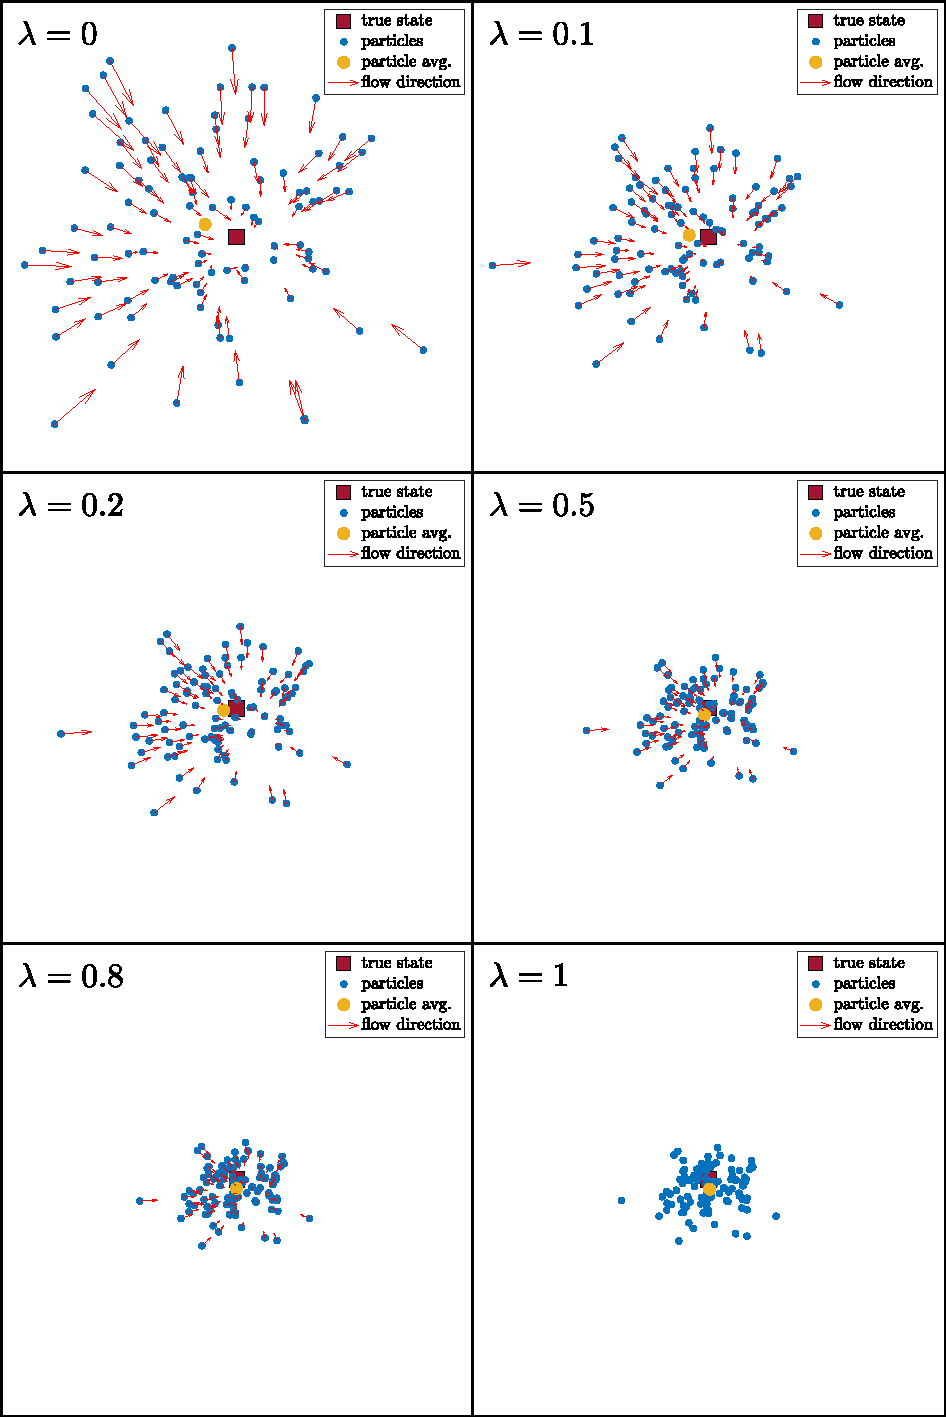
\includegraphics[width=0.98\linewidth]{DHF-visu1.pdf}
    \caption{The particle flow of the DHF (calculated using the exact flow simplification). The time is at a fixed value, while the homotopy is performed from $\lambda = 0$ to $\lambda = 1$.}
    \label{fig:dhf-ill}
\end{figure}

\subsubsection{Other Daum--Huang Filter realizations}

Solving \eqref{eq:dhf-eq} requires various simplifications. Assuming exact flow, where the diffusion part is neglected (only deterministic flow is considered), the measurement model is linear (or linearized), and the noise acting on the system is a Gaussian random variable (or from the exponential family) is only one variation of the Daum--Huang filter. When the linearization of the measurement function is performed around the location of \emph{each} particle instead of their average, the local exact flow Daum--Huang filter is constructed \cite{EDH-Coates}. Particle weighting can be developed for Daum--Huang filters as well, proposed in \cite{pfpf_coates}.

Another simplification is the assumption of incompressible flow \cite{dhf_first}  (this was the first type of the Daum--Huang filter), the assumption of geodesic flow \cite{geodesic}, and the latest results are from the consideration of stochastic particle flow (the diffusion term is no longer neglected), using Gromov's method \cite{gromov}.

It is difficult to summarize the performance of Daum--Huang filters, so is the case with particle filters. Many realizations exist, each with they own advantages and disadvantages. The main problem is with computational capacity: a method with much more advanced and/or more precise calculations can yield better results at a cost of computational time. The main challenge is to develop algorithms and variations that does not require significantly more computation, yet result in a more stable and precise estimation of the state.

\bibliography{library}

\end{document}
